\documentclass[../main.tex]{subfiles}

\graphicspath{{\subfix{../images/}}}

\begin{document}

\section{Task 4}

\begin{enumerate}
    \item Create three global variables of the data structure \texttt{vectorArray} called \texttt{pInst}, \texttt{aInst} and \texttt{bTInst}.
    \item Implement a function called \texttt{setInputMatrices} that fills out the data structures with the input matrix values below.
$$
\text{aInst} = 
\begin{bmatrix}
1  & 2  & 3  & 4  \\
5  & 6  & 7  & 8  \\
9  & 10 & 11 & 12 \\
13 & 14 & 15 & 16
\end{bmatrix}
,\hspace{20pt}
\text{bTInst} = 
\begin{bmatrix}
1 & 1 & 1 & 1 \\
2 & 2 & 2 & 2 \\
3 & 3 & 3 & 3 \\
4 & 4 & 4 & 4
\end{bmatrix}^T
$$
    \item Implement a function called \texttt{displayMatrix} that displays a 4x4 matrix via the USB-UART interface. Test it on matrix \texttt{aInst} or \texttt{bTInst}.
    \item Implement a function called \texttt{multiMatrixSoft} that computes the 4x4 matrix product of the expression $P = A \times B^T$.
    \item Add a command called \texttt{mult} that multiplies \texttt{aInst} and \texttt{bTInst} matrices with the values above. Display the result P and the execution time (in clock ticks) of the function \texttt{multiMatrixSoft} in the USB-UART window.
\end{enumerate}

\subsection*{Solution}

We define the required functions, as well as the \texttt{vectorType} and \texttt{vectorArray} in a header.

\begin{myminted}{matrixMultiplication.h}
#ifndef MATRIXMULTIPLICATION_H
#define MATRIXMULTIPLICATION_H

#include <stdio.h>
#include <xil_printf.h>

#define MATRIX_SIZE 4

typedef union {
    unsigned char comp[MATRIX_SIZE];
    unsigned int vect;
} vectorType;

typedef vectorType vectorArray[MATRIX_SIZE];
vectorArray aInst, bTInst, pInst;

void setInputMatrices(vectorArray matrixA, vectorArray matrixB);
void displayMatrix(vectorArray matrix);
void multiplyMatricesSoft(vectorArray matrixA, vectorArray matrixB, vectorArray matrixP);
void multiplyMatricesHard(vectorArray matrixA, vectorArray matrixB, vectorArray matrixP);

#endif //MATRIXMULTIPLICATION_H
\end{myminted}

\newpage

The \texttt{setInputMatrices} function is shown below. It simply iterates through all the elements of the matrices and assigns the values as specified in the task description.

\begin{myminted}{matrixMultiplication.c - setInputMatrices()}
void setInputMatrices(vectorArray matrixA, vectorArray matrixB)
{
    for (int row = 0; row < MATRIX_SIZE; row++) {
        for (int col = 0; col < MATRIX_SIZE; col++) {
            matrixA[row].comp[col] = MATRIX_SIZE * row + 1 + col;
            matrixB[row].comp[col] = row + 1;
        }
    }
}
\end{myminted}

The \texttt{displayMatrix} function is more or less the same, except it prints the values of the matrix to the UART interface.

\begin{myminted}{matrixMultiplication.c - displayMatrix()}
void displayMatrix(vectorArray matrix)
{
    for (int row = 0; row < MATRIX_SIZE; row++)  {
        for (int col = 0; col < MATRIX_SIZE; col++) {
            xil_printf("%d\t", matrix[row].comp[col]);
        }
        xil_printf("\r\n");
    }
}
\end{myminted}

Lastly the \texttt{multiplyMatricesSoft} function is shown below. Like the previous functions it is a nested loop. Calculating the matrix product of $A$ and $B^T$ and storing the result in $P$.

\begin{myminted}{matrixMultiplication.c - multiplyMatricesSoft()}
void multiplyMatricesSoft(vectorArray matrixA, vectorArray matrixB, vectorArray matrixP)
{ 
    for (int row = 0; row < MATRIX_SIZE; row++) {
        for (int col = 0; col < MATRIX_SIZE; col++) {
            matrixP[row].comp[col] = 0;
            for (int i = 0; i < MATRIX_SIZE; i++) {
                matrixP[row].comp[col] += matrixA[row].comp[i] * matrixB[col].comp[i];
            }
        }
    }
}    
\end{myminted}

\newpage

Finally we add an example function using soft matrix multiplication to our main application. The function \texttt{matrix\_soft} is called when the user inputs '3' in the main menu. The \texttt{matrix\_soft} function should only be called once, so the \texttt{TimerFunctionPtr} is set to \texttt{NULL}. The timer is set to 1 second and started. We will read the counter register in the timer to calculate the number of clock cycles used to perform the matrix multiplication.

\begin{myminted}{main.c - Soft Matrix Multiplication Switch Case}
    case '3':
        xil_printf("\r\nStarting Program 3.");
        xil_printf("\r\nSoft Matrix Multiplication.");
        TimerStop(&TimerInstance);
        TimerFunctionPtr = NULL;
        TimerLoad(&TimerInstance, 1000*MILLISECOND);
        TimerStart(&TimerInstance);
        matrix_soft();
        break;
\end{myminted}

The \texttt{matrix\_soft} function is shown below. It initializes the matrices, displays them, multiplies them and displays the result. The clock cycles are calculated by subtracting the end value from the start value.

\begin{myminted}{main.c - matrix\_soft()}
void matrix_soft()
{
    vectorArray matrixA, matrixB, matrixP;
    u32 start, end;

    setInputMatrices(matrixA, matrixB);

    xil_printf("\r\n\nMatrix A:\r\n");
    displayMatrix(matrixA);

    xil_printf("\r\n\nMatrix B:\r\n");
    displayMatrix(matrixB);

    start = XScuTimer_GetCounterValue(&TimerInstance);
    multiplyMatricesSoft(matrixA, matrixB, matrixP);
    end = XScuTimer_GetCounterValue(&TimerInstance);

    xil_printf("\r\n\nMatrix P (Result of multiplication):\r\n");
    displayMatrix(matrixP);

    /* Subtract 'end' from 'start' since XScuTimer is down counting */
    xil_printf("Clock cycles: %llu\n", 2 * (start - end));
}
\end{myminted}

\newpage

The output of the program is shown below. The matrices are displayed, the product is calculated and displayed, and the number of clock cycles used to perform the matrix multiplication is shown. We see that it takes 3558 clock cycles to perform the matrix multiplication. The Cortex-A9 core is clocked at 650 MHz, meaning the total time for calculating matrix P is:

$$ \frac{3558}{650 * 10^6} = 5.48 \mu s $$

\begin{figure}[h]
    \centering
    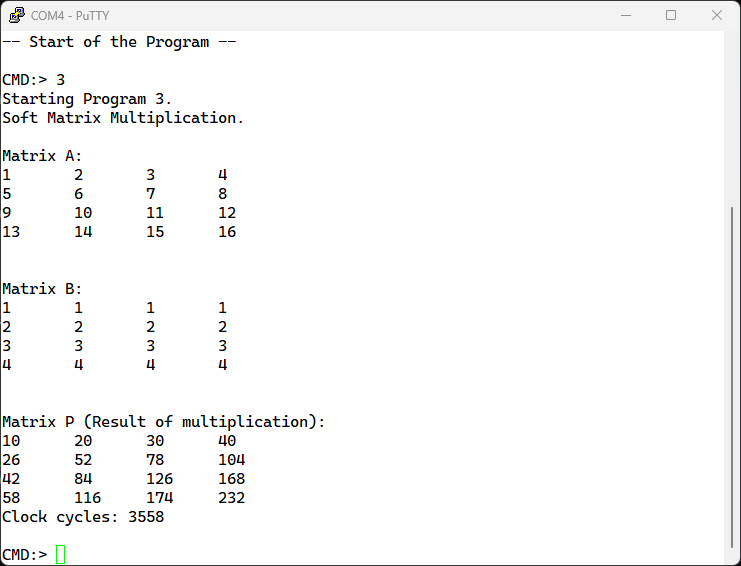
\includegraphics[width=1\textwidth]{task4_putty.png}
\end{figure}


\end{document}